\section{RQ2: Implementations} \label{sec:implementations}

\textit{How are RBAC extension models implemented by their authors?}
\\

When designing and proposing a model targeted at a feature that is rooted in practical
usage by real software systems, implementing the model is evidence that the
proposed model can work in practice. The presence of an actual implementation substantiates the robustness of the design and/or the need for the extension.
We analyzed the primary sources to see how many
proposed models actually had implementations associated with them.
We quantified whether the implementation was an enterprise implementation (i.e., an implementation used in a production environment for a real system) or a prototype implementation (i.e., proof of concept to demonstrate the feasibility). In scientific research software life cycle, NuNamaker et al.~\cite{nunamaker1990systems} illustrated three implementation stages: prototype, enterprise (i.e., product), and technology transfer. Researchers often conduct their research by building a prototype implementation. A prototype implementation serves as a proof of concept to verify that certain concepts of proposed RBAC extension models. The prototype implementation demonstrates feasibility. However, this prototype implementation does not represent a deliverable real-world application. Majority of implementations in RBAC research stops with prototyping. After prototypes are successfully demonstrated, researchers make an effort to further develop a prototype implementation into an enterprise implementation. An enterprise implementation is a deliverable real-world application and allows to conduct realistic evaluations of the RBAC extension models. Technology transfer means that the technology of the proposed RBAC extension models are eventually transferred to the public marketplace. We found that none of implementations of the primary sources reach to the stage of the transfer of technology.


\subsection{Results}

Table \ref{tab:implementations} shows the breakdown of implementations found within the primary sources.
Of the 27 papers surveyed, RBAC extension models in four papers were prototypes developed by the authors whereas RBAC extension models in three papers were claimed to be implemented within a real
system. The remaining 20 papers provide no
mention of an implementation.  

\begin{table}
\centering
\caption{Implementation types found and the count of primary sources}
\vspace{0.1 in}
\begin{tabular*}{.9\linewidth}{| l | p{.5\linewidth} | r | }
\cline{1-3}

\textbf{Implementation Type} & \textbf{Papers} & \textbf{Count} \\ \cline{1-3}
Enterprise
&
\cite{motta03:contextual}
\cite{aich09:role}
\cite{yao2008task}
&
3 \\ \cline{1-3}
Prototype
& 
\cite{cholewka00:acontext-sensitive}
\cite{huang06:pervasive}
\cite{bao08:role}
\cite{zhou2007team}
&
4 \\ \cline{1-3}
None
&
\cite{ni2010privacy}
\cite{jian2008extended}
\cite{alam06:constraint}
\cite{tzelepi01:flexible}
\cite{yamazaki04:designing}
\cite{thein2011leveraging}
\cite{zou2009crbac}
\cite{haibo05:context}
\cite{zhang06:collaborative}
\cite{masoumzadeh2008purbac}
\cite{damiani2007geo}
\cite{ray2006lrbac}
\cite{hansen2003spatial}
\cite{aich07:STARBAC}
\cite{chen08:spatio-temporal}
\cite{samuel07:spatio-temporal}
\cite{chandran05:llt}
\cite{ray07:spatio}
\cite{oh2003task}
\cite{joshi05:generalized}
&
20 \\

\cline{1-3}
\end{tabular*}
\label{tab:implementations}
\end{table}

\subsection{Analysis and Discussion}

The RBAC standard is designed such that when practitioners implemented RBAC into their systems, the RBAC standard demonstrates reasonable assurance being based off a well thought out model.
As extensions to the RBAC Reference Mode come along, thought and time would be given to how features and nuances of their models may impact implementation to achieve the same goals as the original standard. 
The primary sources showed a lack of implementation
with over 70\% of the models having no notion of attempting to implement them. Prototype implementation shows the feasibility of the RBAC extension models in the four papers. Of the models that produced an implementation within the enterprise world, two were from within the medical domain and one was implemented using web application technologies.  


\greybox{Research on RBAC extension models shows a lack of implementations in the real world scenarios that the models are ultimately designed for.}

\section{RQ3: Evaluations} \label{sec:evaluations}

\textit{How are RBAC extension models evaluated by their authors?}
\\

The 27 primary sources were examined for evidence that evaluations of the proposed model were presented by the model authors. 
Zelkowitz and Wllace~\cite{Zelkowitz1998experimentalmodels} proposed evaluation types and methods that are used to validate the claims in the paper. 
Table~\ref{tab:evaluationtypes} illustrates 12 evaluation methods with their corresponding general evaluation types and descriptions. We classified each paper according to the evaluation methods shown in Table~\ref{tab:evaluationtypes}. For example, Aich et al. conducted project monitoring to show the performance and complexity of their proposed RBAC extension model \cite{aich09:role}.



\subsection{Results}

Table~\ref{tab:evaluations} shows evaluation methods and criteria.
Based on the diverse evaluation methods, 12 models presented no evidence of an evaluation. Fourteen models presented 
example scenarios and how application of their model would apply and resolve the situation. These methods refer to assertions.
Six models provided some form of performance
or complexity analysis of their model through project monitoring.  The performance and complexity analysis included graphs of the model's time to determine calculate authorization 
as the number of entities grew, and the size of the role space for the extension model compared to the RBAC Reference Model. 
Five models provided simulations based on mathematical descriptions and analysis as a way to provide evaluation in the form of completeness. 
The most widely used evaluation method was assertion, which provides sample scenarios with accompanying workflows of how the extension model
would tackle those scenarios.
%Much is left to the reader to assume of these types of evaluations, as the authors do not explicitly state
%or show how the Reference Model is deficient in tackling said scenarios.

% Table generated by Excel2LaTeX from sheet 'Sheet1'
\begin{table}[t]
  \centering
  \caption{Evaluation Types and methods classified by Zelkowitz and Wllace~\cite{Zelkowitz1998experimentalmodels}}
  %  \begin{tabular}{|l|l|l|}
   \begin{tabular*}{.9\linewidth}{| p{.25\linewidth}| p{.2\linewidth} | p{.35\linewidth} |}
		\hline
			
    \textbf{Evaluation Type} & \textbf{Method} & \textbf{Description} \\\hline
			
    \multirow{4}[8]{*}{Observational methods} & Project monitoring & Monitor project and collect development data \\\cline{2-3}
          & Case study & Monitor project in depth and collect data with a specific goal for the project \\\cline{2-3}
          & Assertion & This evaluation uses examples for validation\\\cline{2-3}
          & Field study & Monitor multiple projects and collect relevant information to compare the projects \\\hline
    \multirow{3}[6]{*}{Historical methods} & Literature research & Examine previously published projects \\\cline{2-3}
          & Legacy & Examine data from completed projects \\\cline{2-3}
          & Lessons learned & Examine qualitative data from projects \\\hline
    \multirow{5}[10]{*}{Controlled methods} & Static analysis & Examine structure of dveloped product \\\cline{2-3}
          & Replicated experiment & Develop mulitple versions of product \\\cline{2-3}
          & Synthetic environment & Replicate one factor in laboratory setting \\\cline{2-3}
          & Dynamic analysis & Execute developed product for perormance \\\cline{2-3}
          & Simulation & Execute product using a model of real enviroment \\\hline
   
    \end{tabular*}%
  \label{tab:evaluationtypes}%
\end{table}%


\begin{table}
\centering
\caption{Evaluation methods by primary source}
\vspace{0.1 in}
\begin{tabular*}{.9\linewidth}{| p{.2\linewidth}| p{.35\linewidth} | p{.2\linewidth} | r | }
\cline{1-4}
\textbf{Methods} & \textbf{Criteria} & \textbf{Papers} & \textbf{Count} \\ \cline{1-4}
\multirow{2}[0]{*}{Project Monitoring}
&
Time-Based Performance
&
\cite{ni2010privacy}
\cite{aich09:role}
&
2 \\ \cline{2-4}

&
Complexity Analysis
&
\cite{bao08:role}
\cite{zhang06:collaborative}
\cite{aich07:STARBAC}
\cite{chen08:spatio-temporal}
&
4 \\ 
\cline{1-4}
Case Study
&
RBAC Model in Practice
&
\cite{motta03:contextual}
&
1 \\ \cline{1-4}
Assertion
&
Example Scenarios of the Model in Action
&
\cite{jian2008extended}
\cite{yao2008task}
\cite{cholewka00:acontext-sensitive}
\cite{huang06:pervasive}
\cite{bao08:role}
\cite{zhou2007team} 
\cite{alam06:constraint}
\cite{tzelepi01:flexible}
\cite{yamazaki04:designing}
\cite{zou2009crbac}
\cite{samuel07:spatio-temporal}
\cite{ray07:spatio}
\cite{joshi05:generalized}
\cite{oh2003task}
&
14 \\ \cline{1-4}
Field Study
&
Comparison to Standard RBAC
&  
\cite{bao08:role}
\cite{zou2009crbac}
\cite{zhang06:collaborative}
\cite{ray07:spatio}
\cite{zhao2008flexible}
&
5 \\ \cline{1-4}
Simulation
&
Mathematical Modeling
&  
\cite{damiani2007geo}
\cite{hansen2003spatial}
\cite{aich07:STARBAC}
\cite{chen08:spatio-temporal}
\cite{joshi05:generalized}
&
5 \\ \cline{1-4}
No Evaluations
&
Not Applicable
&
\cite{masoumzadeh2008purbac}
\cite{ray2006lrbac}
\cite{chandran05:llt}
&
3 \\ \cline{1-4}

\end{tabular*}
\label{tab:evaluations}
\end{table}

\subsection{Analysis and Discussion}

  
When proposing an access control model, providing an evaluation of the model is a key component in establishing the validity of the model. 
Further, in the case of extensions to the RBAC Reference Model, the model is accompanied by validation of the model as a stand-alone
access control model and in comparison to the model upon which the enhancements are being made. The results show that robust evaluations of
extension models are lacking. 

The primary source of validation a developer or practitioner may encounter is a qualitative discussion of real-world
scenarios and how the proposed model can tackle those situations. 
For five of the primary sources \cite{bao08:role} \cite{zou2009crbac} \cite{zhang06:collaborative} \cite{ray07:spatio} \cite{zhao2008flexible}, the model authors conduct field study to provide some discussion of how the RBAC Reference Model is deficient in tackling the scenario.
In Table \ref{tab:evaluations}, we observe that one paper includes a case study to examine how the proposed model works in practice. Discussions
of how an extension model handles a real-world scenario provides developers and practitioners anecdotal evidence at best
for what types of situations the proposed model could handle. Further, by not providing a comparison to the RBAC Reference Model, developers may be left implementing a more complex model to address their requirements when the RBAC Reference Model would
have sufficed.  Further, given the nature of access control models as grounded in application to enterprise implementations, 
case studies of a model in action provide developers with evidence that the model works as intended when applied.

When looking for an enterprise ready access control mechanism, developers must balance usability with security. 
Two of the primary sources examined provided time-based performance analysis of their extension model compared
to the RBAC Reference Model through project monitoring. This inclusion of time analysis provides some assurances to developers that any non-functional
requirements surrounding time to compute authorizations compete or beat the RBAC Reference Model. Further, four of the models provided
some form of complexity of their model through project monitoring. This complexity analysis plays a key role in the management of the access control mechanism
over the course of the models implementation lifetime. As the number of roles, users and additional entities grows, developers will 
need to ensure non-functional requirements are met that deal with the ability for a system administrator to effectively manage these
entities.

\greybox{RBAC extension model research lacks comprehensive evaluation of the models both in theory and in practice.}


\section{RQ4: Domains} \label{sec:domains}

\textit{What domains have been targeted by RBAC extension models?}
\\

Business needs have historically driven RBAC research and development.  The primary mode of evaluation for
model extensions has been the presentation of business scenarios in various domains and how the model
uniquely handles those particular scenarios.  Thus, looking for trends in the domains used in the example
scenarios might serve to illuminate a trend worth further examination into the reason for the explosion of
RBAC extensions.  We identified domains presented within the primary sources by looking for example
scenarios cast within a particular domain or mention of domain requirements within the body of the paper.

\subsection{Results}

Table \ref{tab:domains} shows domains mentioned and their associated sources.

\begin{table}
\centering
\caption{Domains by primary source}
\vspace{0.1 in}
\begin{tabular*}{.9\linewidth}{| p{.45\linewidth} | p{.3\linewidth} | r | }
\cline{1-3}

\textbf{Domain} & \textbf{Papers} & \textbf{Count} \\ \cline{1-3}
Medical Domain
&
\cite{ni2010privacy}
\cite{motta03:contextual}
\cite{aich09:role}
\cite{zhou2007team}
\cite{alam06:constraint}
\cite{tzelepi01:flexible}
\cite{damiani2007geo}
\cite{hansen2003spatial}
\cite{samuel07:spatio-temporal}

&
9 \\ \cline{1-3}
Pervasive Computing Environments
& 
\cite{huang06:pervasive}
\cite{ray07:spatio}
\cite{chen08:spatio-temporal}
&
3 \\ \cline{1-3}
Web Applications
&
\cite{haibo05:context} 
\cite{masoumzadeh2008purbac}
&
1 \\ \cline{1-3}
Mobile Computing
&
\cite{aich09:role} 
\cite{thein2011leveraging}
\cite{zou2009crbac}
\cite{ray2006lrbac}
\cite{chandran05:llt}
&
4 \\ \cline{1-3}
Organizations with Many Sub-departments
&
\cite{yao2008task} 
\cite{yamazaki04:designing}
&
2 \\ \cline{1-3}
Enterprise Workflows
&
\cite{cholewka00:acontext-sensitive}
\cite{bao08:role}
\cite{zhang06:collaborative}
\cite{oh2003task}
\cite{joshi05:generalized}
&
5 \\ \cline{1-3}
None
&
\cite{jian2008extended}
\cite{aich07:STARBAC}
&
2 \\ \cline{1-3}

\end{tabular*}
\label{tab:domains}
\end{table}

The predominant domain for which extension models have been generated for is that of the medical domain with 9 of 27 mentioning scenarios or requirements of that industry.
Mobile computing and enterprise workflows were each represented by five papers claiming to be influenced by the requirements for access control within these domains. The final set
of domains was pervasive computing environments and large-scale organizations with three each and web applications with one.  Two papers~\cite{jian2008extended, aich07:STARBAC} do not mention domains explicitly since Aich et al. \cite{aich09:role} fall under both the medical domain and mobile computing.

\subsection{Analysis and Discussion}

The medical domain produced the largest selection of papers when analyzing the domains influencing the proposals of RBAC extension models.  
Moreover, we observed that the categories associated with papers identifying the medical domain were not limited to one or two but cut across
each of the eight categories except for the Organizational category. 
The cross-category nature of the medical domain papers appears indicative of the complex nature of medical applications and requirements.
Given the growth of the research and development of medical applications over the past decade this result does not appear to be surprising. However,
the RBAC standard was originally created to reduce cost and increase interoperability - two goals of current regulation around the standardization
of electronic health record systems. The large number of proposed models, and the cross-category result stand in direct opposition of the goals
of both the RBAC standard and current regulations.

The RBAC standard has been re-enforced by the economic impact that standardization has had on enterprises needing to apply access control.  The
inclusion of extension models targeted at the enterprise workflow domain is indicative of the expansion of requirements for enterprises. Developers
and researchers would take care when looking at extension models designed to address the newer requirements of enterprise workflows to
achieve the same economic implementation and maintainability benefits the RBAC Reference Model presents.

Figure~\ref{fig:dist_domains} shows domain distribution by 3-year period.
We observed that medical and enterprise domain papers constantly appear for every period in Figure~\ref{fig:dist_domains}.
For a domain that has roots in medical and enterprise computing, protecting the data of both through access controls is paramount given their ubiquity. 
Mobile computing has seen a dramatic increase in the number of available devices, operating systems and applications since 1997 when the first smart phone was introduced \cite{buck2013new}. Since 2004, the domain analysis results produced five papers that targeted extensions that are designed to address the requirements of mobile computing. 

\greybox{RBAC extension models were found targeting domains such as medical, pervasive computing, web applications, enterprise workflows and mobile computing.}

\begin{figure}[ht]
    \centering
        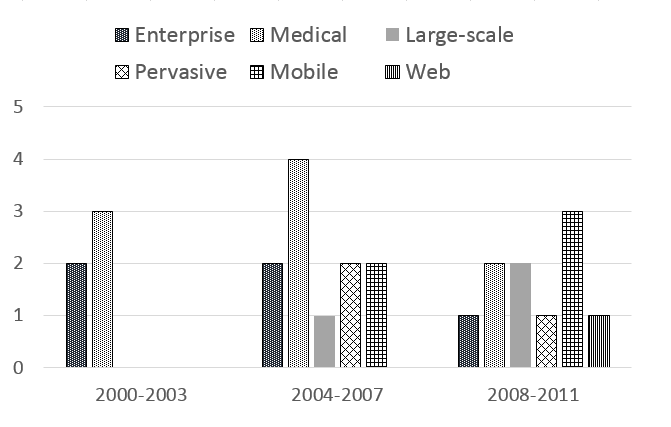
\includegraphics[width=4.0in]{sections/dist_domains_byYear.png}
\vspace{-0.2 in}
    \caption{\label{fig:dist_domains}Domain distribution by 3-year period. Y-axis represents the number of corresponding domain papers.
    X-axis represents 3-year period from 2000 to 2011.}
\end{figure}

\section{RQ5: Generalizations} \label{sec:generalizations}

\textit{What commonalities exist across RBAC extension models?}
\\

During the paper reading phase, we identified commonalities within the primary sources
by looking for formal modeling of extending RBAC extension models.

\subsection{Results}

The RBAC standard is used in various aspects of computer systems. To reduce efforts for modeling access control used in various applications, researchers often focus on developing generalized core concepts of access control.
The authors use formal model to provide high level description of access control model across all categorizations.
Formal model of access control provides precise understanding, specification, and analsysi of access control.
Formal model~\cite{abadi2008variations} of access control can be specified in one of logic expressions such as propositional logic. For example, in propositional logic, simple (i.e., atomic) or compound condition at given context is evaluated to true or false based on specified rules and access control logic. Aich et al.~\cite{aich09:role} proposed STARBAC model,  which can be expressed in propositional logic. While propositional logic does not support for quantifiers, first-order logic (i.e., predicate logic) extends propositional logic by the use of quantifiers. For example, ESTARBAC model~\cite{aich09:role} can be expressed in first-order logic.


\subsection{Analysis and Discussion}

We found that 27 papers of RBAC extensions provide formal model based on logic expressions to describe its extended model.
%Since NIST proposed RBAC standard using logic expression, we observed that researchers describe extended RBAC models using logic expressions.
We discuss two widely used logic expressions for access control: propositional logic and first-order logic. 
Given context, propositional logic is used to evaluate true or false based on specified rules and access control logic. As access control is typically evaluated to either true or false based on predicates, propositional logic is sufficient to describe key ideas and definitions. Propositional logic is suitable for specifying what combination of attributes values a request must satisfy to be authorized to roles.
However, propositional logic has limitations. While this logic is simple, this logic does not support for quantifiers and reasoning about RBAC, which helps
reduce the administrative complexity of associations such as user- role associations.
To support for reasoning of access control, one may describe the RBAC extended models in first-order logic. First-order logic is expressive enough to concisely represent access control systems.
Given an RBAC extension model, Samuel et al.~\cite{samuel07:spatio-temporal} proposed verification of the model using a specification language, which is based first-order logic. 
This logic is sufficient to model RBAC and extended RBAC for reasoning. 
Moreover, this logic supports for concise and elegant formulation of the Reference Model and its relation. 
 
%First-order logic uses relations, variables, and quantifiers.
 


%Combination of attribute values may handle constraints such as temporal and spatial constraints. For example, we describe user-role authorization as $ae$ $\Rightarrow$ $r$ using propositional logic where $ae$ is an attribute expression and $r$ is a role. Propositional logic for RBAC has two parts. The left hand side (LHS) is an attribute expression $ae$. 
%The right hand side (RHS) is a role. 
%If a request satisfies the attribute expression, a user $u$ in the request is authorized to the role specified in RHS.



.
